\documentclass[conference]{IEEEtran}
\IEEEoverridecommandlockouts
% The preceding line is only needed to identify funding in the first footnote. If that is unneeded, please comment it out.
\usepackage{cite}
\usepackage{amsmath,amssymb,amsfonts}
\usepackage{algorithmic}
\usepackage{graphicx}
\usepackage{textcomp}
\usepackage{xcolor}
\usepackage{color}
\usepackage{listings}
\usepackage{xparse}
\usepackage[spaces,hyphens]{url}
\usepackage{hyperref}

\def\BibTeX{{\rm B\kern-.05em{\sc i\kern-.025em b}\kern-.08em
    T\kern-.1667em\lower.7ex\hbox{E}\kern-.125emX}}
    
\NewDocumentCommand{\codeword}{v}{%
\texttt{\textcolor{blue}{#1}}%
}

\NewDocumentCommand{\tool}{v}{%
\texttt{\textcolor{gray}{#1}}%
}

\lstset{language=Bash,keywordstyle={\bfseries \color{blue}}}

\hypersetup{
    colorlinks=true,
    linkcolor=blue,
    filecolor=magenta,      
    urlcolor=cyan,
    pdftitle={Overleaf Example},
    pdfpagemode=FullScreen,
    }
    
\definecolor{dkgreen}{rgb}{0,0.6,0}
\definecolor{gray}{rgb}{0.5,0.5,0.5}
\definecolor{mauve}{rgb}{0.58,0,0.82}

\lstset{frame=tb,
  language=Bash,
  aboveskip=3mm,
  belowskip=3mm,
  showstringspaces=false,
  columns=flexible,
  basicstyle={\small\ttfamily},
  numbers=none,
  numberstyle=\tiny\color{gray},
  keywordstyle=\color{blue},
  commentstyle=\color{dkgreen},
  stringstyle=\color{mauve},
  breaklines=true,
  breakatwhitespace=true,
  tabsize=3
}

\begin{document}

\title{OMNet++ dengan Algoritma Dijkstra}

\author{\IEEEauthorblockN{Agil Seftian}
	\IEEEauthorblockA{\textit{Teknik Komputer, Fakultas Teknologi Informasi} \\
		\textit{Institut Teknologi Batam}\\
		Batam, Indonesia \\
		1922016@student.iteba.ac.id}
	\and
	\IEEEauthorblockN{Rizky Sandiary}
	\IEEEauthorblockA{\textit{Teknik Komputer, Fakultas Teknologi Informasi} \\
		\textit{Institut Teknologi Batam}\\
		Batam, Indonesia \\
		1922014@student.iteba.ac.id}
}
\maketitle

\begin{abstract}
	OMNeT ++ adalah framework dan library simulasi C ++ berbasis komponen, terutama untuk membangun simulator jaringan. Ini merupakan UAS Jaringan komputer dan kami mencoba sebuah simulasi jarigan.

\end{abstract}

\begin{IEEEkeywords}
	Omnet++, Simulasi, Dijkstra
\end{IEEEkeywords}

\section{Pendahuluan}
Ini merupakakn Tugas UAS Jaringan Komputer, paper ini bertujuan untuk memandu mahasiswa dalam membuat dan bekerja dengan contoh model simulasi.

\subsection{Algoritma Dijkstra}
Dijkstra adalah algoritma yang digunakan untuk mencari lintasan terpendek pada sebuah graf berarah. Contoh penerapan algoritma ini adalah lintasan terpendek yang menghubungkan antara dua kota ataupun titik berlainan tertentu. Algoritma Dijkstra bekerja dengan membuat jalur ke satu simpul optimal pada setiap langkah. Jadi pada langkah ke n, setidaknya ada n node yang sudah kita tahu jalur terpendek.
\break
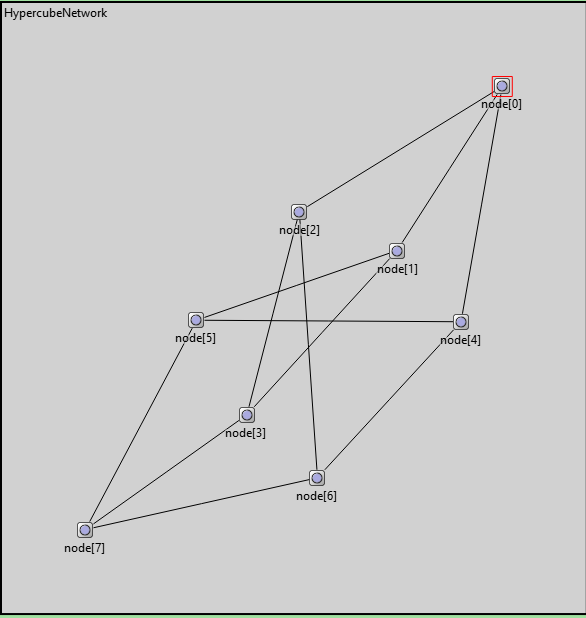
\includegraphics[scale=0.5]{images/algoritma-dijkstra.png}

\section{Pengerjaan}\label{pengerjaan}
Langkah-langkahnya metodologi:

\subsection{Metodologi}

\subsection{Langkah Instalasi}
\begin{enumerate}
	\item Buka official site OMNet++.
	\item Download terlebih dahulu OMNet++ 
	Extract zip yang sudah didownload ke direktori yang diinginkan(nantinya akan menjadi direktori instalasi OMNet++
	\item Buka direktori hasil extract sebelumnya lalu double-click file mingwenv, jalankan perintah configure lalu tunggu hingga selesai. Setelah itu jalankan perintah make dan tunggu hingga selesai.
	\item Setelah itu kita dapat membuka IDE dengan mengetikkan perintah omnetpp di terminal mingwenv. Dan proses instalasi selesai
\end{enumerate}


\subsection{Flowchart}
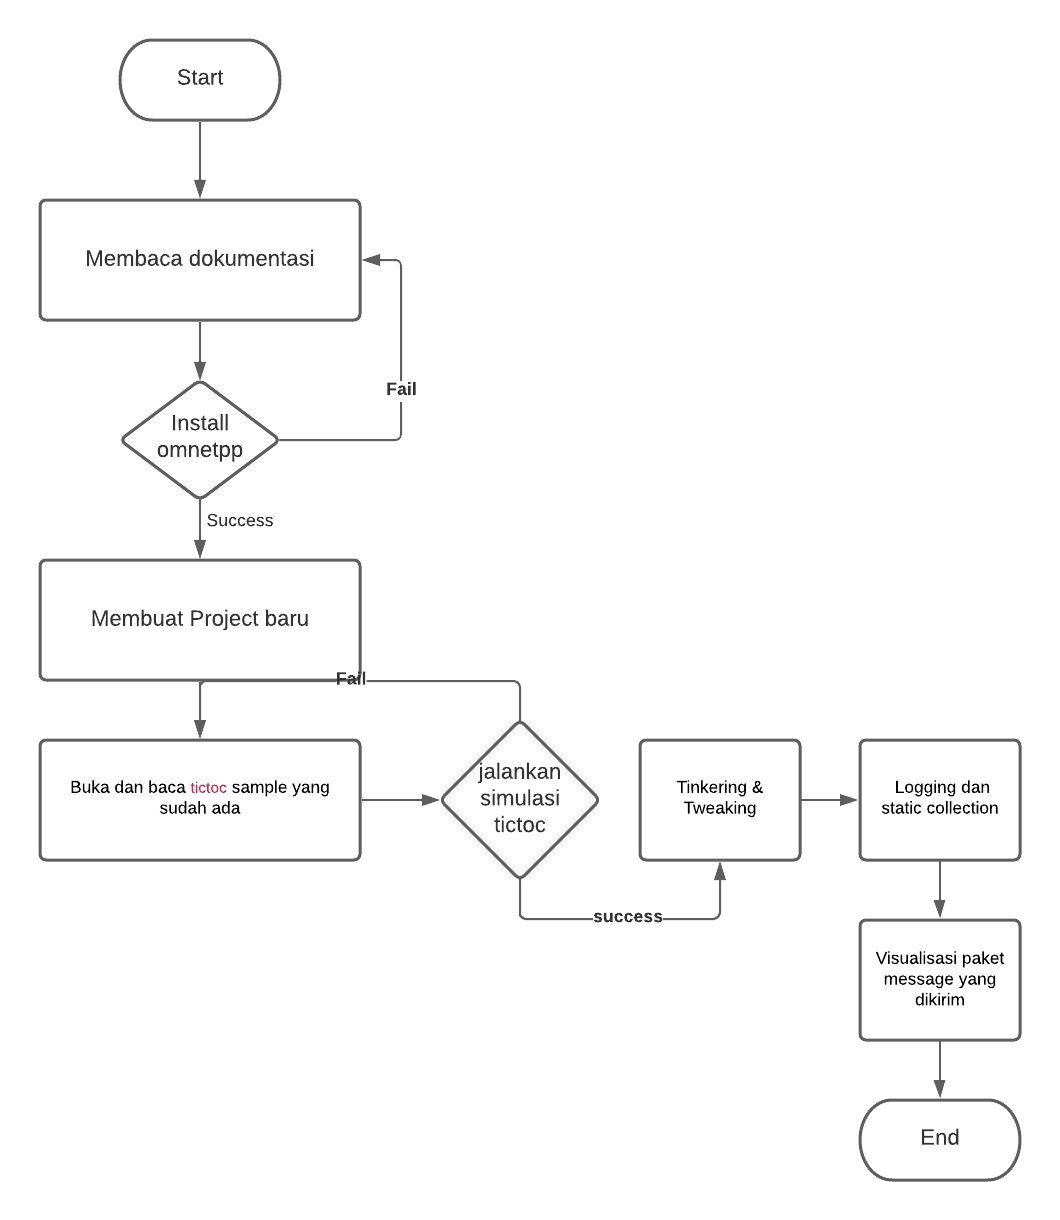
\includegraphics[scale=0.18]{images/flowchart.png}

\section{Scenario}
Sebuah hypercube dengan dimensi d memiliki \(2^d\) node. Jika kita memberi nomor pada simpul dari 0 hingga \(2^d-1\) dan lihat angkanya sebagai biner d-digit nomor, maka setiap node akan terhubung ke d node lain yang berbeda hanya dalam satu bit. Artinya, misalkan d=4 misalnya, maka 0010 (simpul 2) akan terhubung ke 1010 (simpul 10), 0110 (simpul 6), 0000 (0) dan 0011 (simpul 3). Ini adalah bagaimana hypercube dibangun di hcube.ned; gerbang number adalah jumlah bit yang berbeda, yaitu node 0010's gerbang #2 menuju ke simpul 0110. Modul hypercube di hcube.ned mengambil dimensi d sebagai parameter.Itu juga membutuhkan parameter lain yang disebut nodetype: string yang menamai jenis modul yang akan digunakan sebagai simpul di hypercube. Di hc\_net.ned, ketika jaringan hypercube dijelaskan, nodetype memberikan "HypercubeNode" nilai. HypercubeNode adalah tipe modul gabungan yang terdiri dari a sumber lalu lintas (generator), wastafel lalu lintas dan modul router.

Modul router bekerja dengan cara berikut. Ada slot waktu yang semua transmisi disinkronkan. Di setiap slot waktu, node router menerima paket dari tetangganya, memutuskan gerbang mana untuk setiap paket perlu dikirim, dan mengirimkannya di slot waktu berikutnya. Dalam hypercube, perutean sederhana: bilangan biner dari arus node dan node tujuan berbeda dalam  seberapa bit; sedikit kebutuhan untuk 'diperbaiki' dan paket harus dikirim melalui yang sesuai gerbang. Misalnya, jika kita berada di node 0010 dan tujuan paket adalah 1000, maka bit 3 dan bit 1 berbeda, sehingga paket dapat dikirim juga di gerbang 3 atau di gerbang 1. Jadi idealnya, paket apa pun bisa mencapai tujuannya dalam sejumlah hop yang merupakan jarak Hamming antara sumbernya dan nomor node biner tujuan. 

Modul router menggunakan perutean defleksi. Ini berarti tidak ada buffer dalam modul router: jika lebih dari satu paket perlu dikirim melalui gerbang yang sama, lalu yang satu dibelokkan: dikirim keluar melalui gerbang lain. Paket dari pengguna lokal (sumber lalu lintas atau generator) hanya dapat diterima jika ada gerbang bebas yang tersisa di slot waktu yang diberikan, yaitu, kurang dari d paket perlu dirutekan. File hc\_rte.cc berisi: Modul sederhana HCRouter yang mengimplementasikan perutean defleksi sederhana skema. 

\section{Pembahasan}
Bagian ini akan menjelaskan secara singkat mengenai tiap bagian-bagian dari Tutorial Learn OMNeT++ with TicToc. Namun kita tidak perlu mengikuti seluruh bagian yang dijelaskan pada halaman ini, seperti contohnya membuat sample dan menambahkan NED file. Dikarenakan saat kita menginstal sudah disediakan seluruh contohnya pada direktori samples beserta penjelasannya.

\subsection{Part 1: \href{https://docs.omnetpp.org/tutorials/tictoc/part1/}{Getting Started}}
Model pertama yang akan dikerjakan pada tutorial ini adalah model tic-toc, dimana terdapat sebuah node yang saling mengirim dan menerima paket secara berulang. Ketika IDE sudah dibuka akan terlihat seperti gambar berikut,
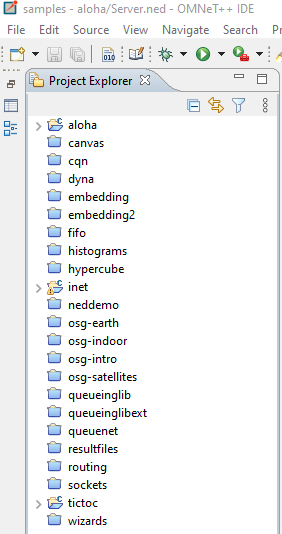
\includegraphics[scale=0.9]{images/samples-directory.png}


lalu buka tictoc folder, didalamnya terdapat banyak sekali file. Pilih tictoc1.ned.

\subsection{Part 2: \href{https://docs.omnetpp.org/tutorials/tictoc/part2/}{Running the Simulation}}
Untuk menjalankan simulasinya, kita dapat menekan tombol \codeword{Run}\break
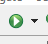
\includegraphics[scale=0.9]{images/run-button.png}

Akan terlihat sebuah \textit{console window} yang akan menjalankan proses \textit{Compiling}. Tunggu beberapa saat lalu akan muncul \textit{window} baru.\break 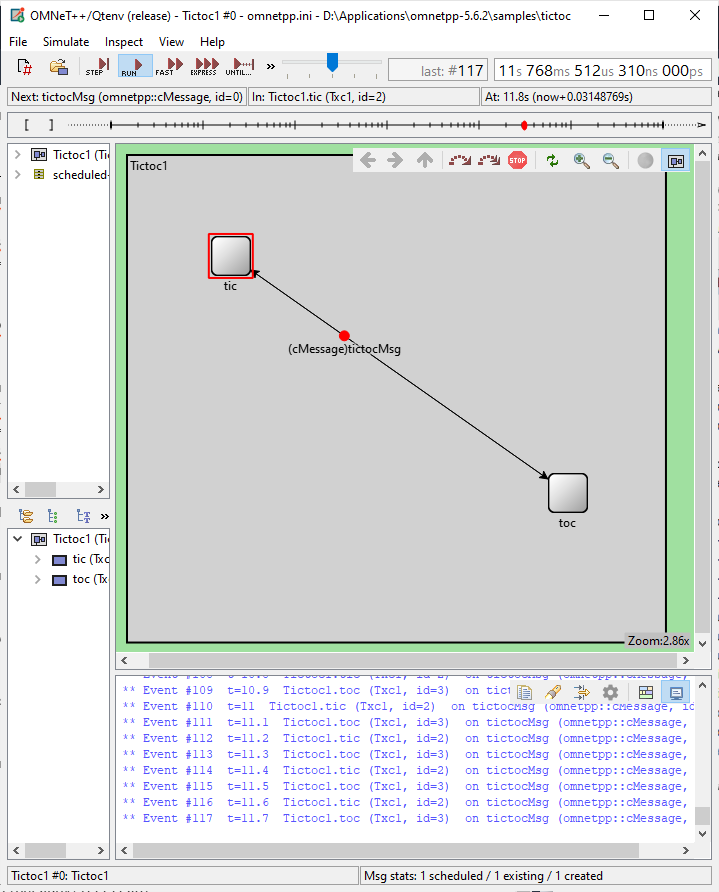
\includegraphics[scale=0.35]{images/simulation-window.png}

Dibagian ini juga kita dapat melakukan beberapa hal lainnya, seperti \textit{Debugging} dan \textit{Logging}, dapat juga memvisualisasikan menggunakan \textit{Sequence Chart}.

\subsection{Part 3: \href{https://docs.omnetpp.org/tutorials/tictoc/part3/}{Enhancing the 2-node TicToc}}
Pada bagian ini kita dapat meningkatkan \textit{2-node TicToc} menggunakan \textit{icon, logging, state variables, parameters, timers, etc}.

Untuk melihat contoh implementasi \textit{icon}, dapat membuka  dan menjalankan \textit{file} \codeword{tictoc2.ned}.\break

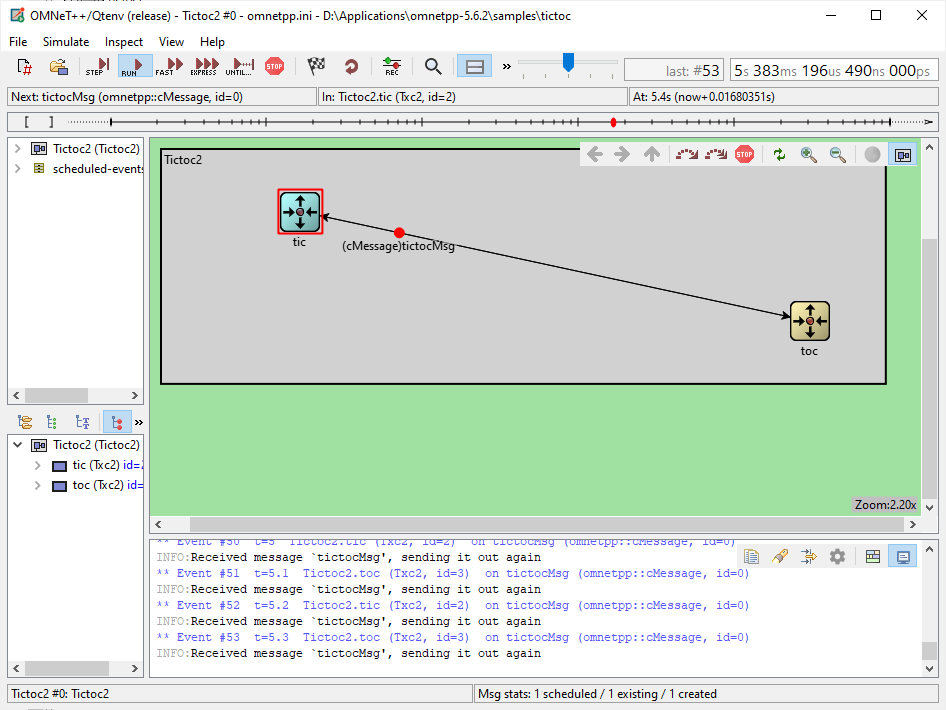
\includegraphics[scale=0.25]{images/tictoc2.ned.png}
\textit{Files:} \codeword{tictoc2.ned}, \codeword{txc2.cc}


untuk melihat contoh implementasi icon, silahkan buka \textit{file} \codeword{tictoc3.ned}. Jalankan simulasi dan klik kanan pada \textit{node}, klik menu \codeword{Open Component Log for 'tic'}. Akan muncul log seperti gambar berikut

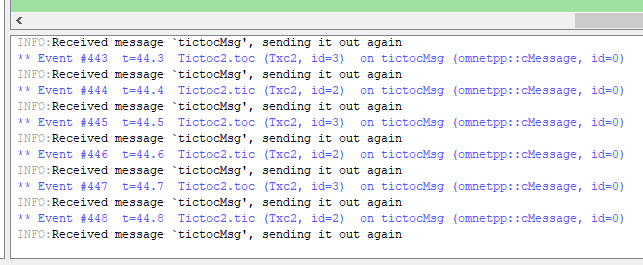
\includegraphics[scale=0.38]{images/tictoc3-log.ned.png}


selain itu terdapat beberapa \textit{file sample} yang dapat kita coba:
\begin{itemize}
	\item Parameters; \textit{Files: }\codeword{tictoc4.ned}, \codeword{txc4.cc}
	\item Timeout, cancelling timers; \textit{Files: }\codeword{tictoc8.ned}, \codeword{txc8.cc}
	\item etc
\end{itemize}

\subsection{Part 4: Turning it Into a Real Network}
Bagian ini akan menampilkan contoh implementasi lebih dari \textit{2 nodes}. Dapat membuka dan menjalankan simulasi \textit{file} \codeword{tictoc10.ned} . Kurang lebih akan terlihat seperti ini.
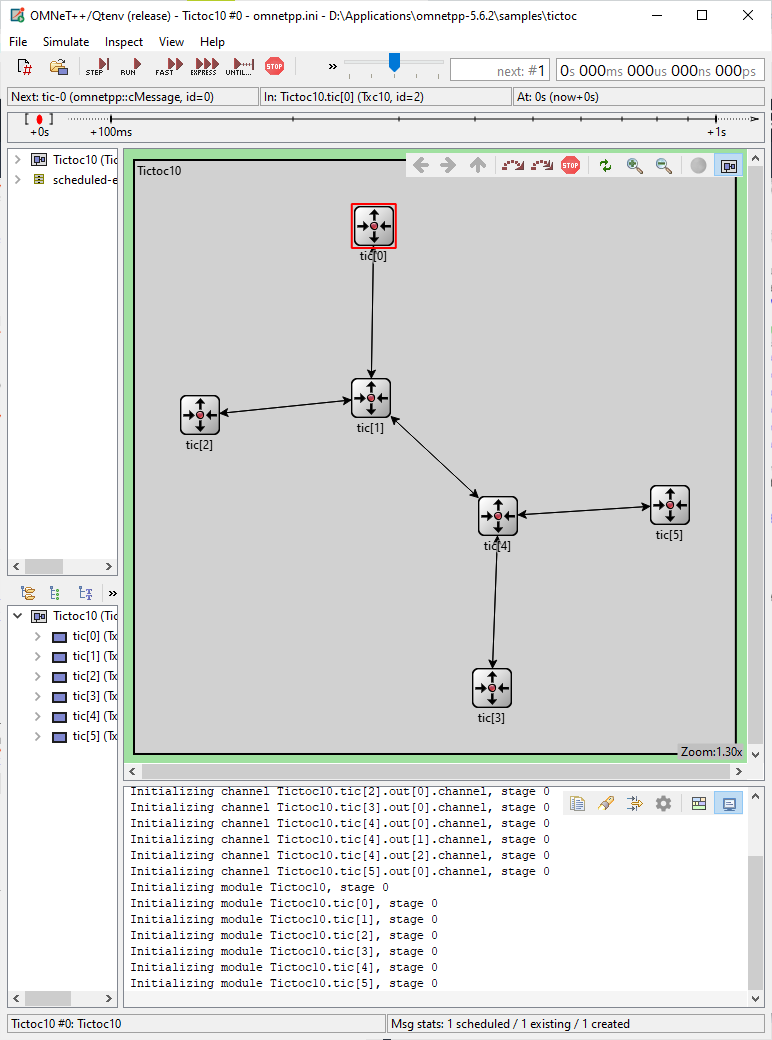
\includegraphics[scale=0.25]{images/tictoc10.ned.png}

\subsection{Part 5: Adding Statistics Collection}
Dari simulasi tersebut kita dapat mengumpulkan statistik data antar node juga. Seperti yang sudah diimplementasi di \codeword{txc14.cc}.

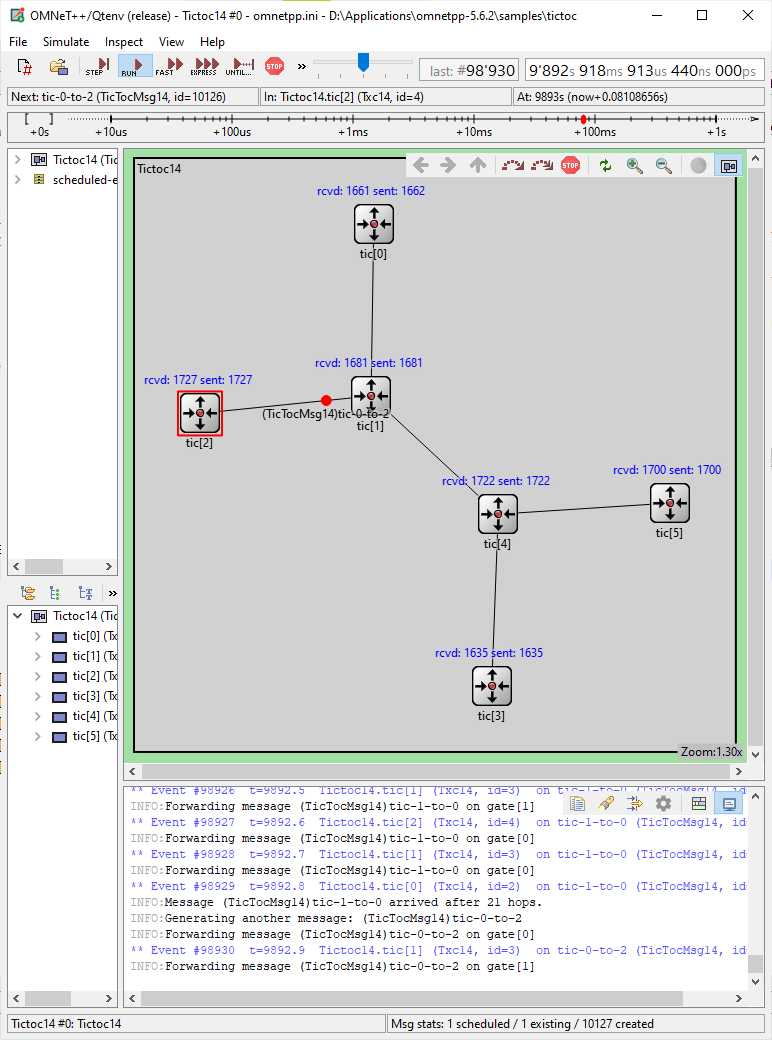
\includegraphics[scale=0.23]{images/tictoc14.ned.png}\break
\textit{Files:} \codeword{tictoc14.ned}, \codeword{tictoc14.msg}, \codeword{txc14.cc}

Kita dapat menampilkan Histogram data dengan cara sebagai berikut:
\begin{enumerate}
	\item Buka dan jalankan simulasi \textit{sample file} \codeword{tictoc15.ned} dengan mode \codeword{Fast} seperti gambar berikut\break
	      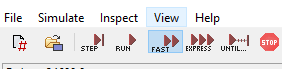
\includegraphics[scale=0.8]{images/fast-mode-button.png}

	\item Klik kanan pada \codeword{tic[1]}, lalu \codeword{Open Details for 'tic[1]'}\break
	      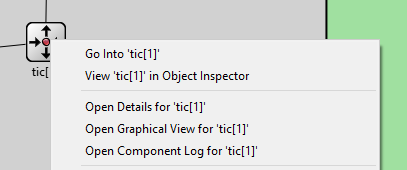
\includegraphics[scale=0.53]{images/tic[1].png}

	\item Setelah itu klik kanan lagi pada \codeword{hopCountStats}, lalu pilih \codeword{Open Graphical View for 'hopCountStats'}.\break
	      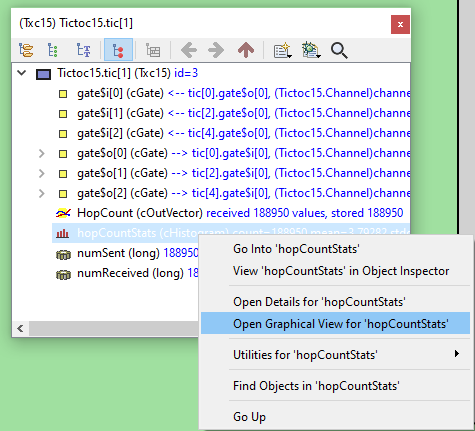
\includegraphics[scale=0.5]{images/tic[1]-histogram.png}. \break

	      Maka akan muncul Histogramnya seperti ini\break
	      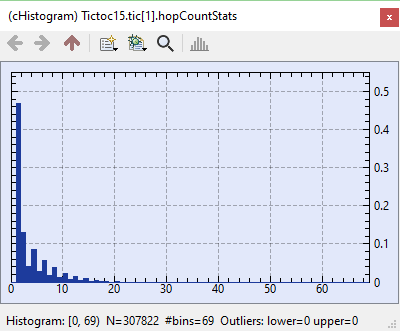
\includegraphics[scale=0.32]{images/tic[1]-histogram2.png}
\end{enumerate}

\subsection{Part 6: Visualizing the Results With the IDE}
Hasil dari \textit{static collection} dapat kita visualisasikan dalam berbagai model \textit{chart}. Berikut cara-caranya:
\begin{enumerate}
	\item Buka \textit{sample file} \codeword{tictoc/results/Tictoc15-#0.sca}
	\item Pada bagian bawah, klik \codeword{Browse Data}
	      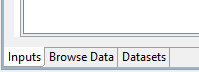
\includegraphics[scale=0.65]{images/browse-data-tab.png}
	      \newpage
	\item Lalu pilih \codeword{Vector} data
	      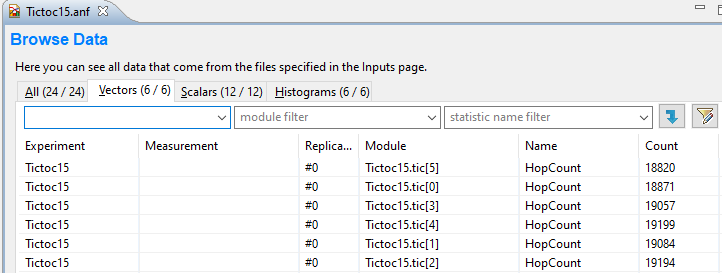
\includegraphics[scale=0.27]{images/vector-data.png}
	\item Lalu \textit{Select all}, klik kanan lalu \codeword{Plot}. Maka akan muncul data visualnya.
	      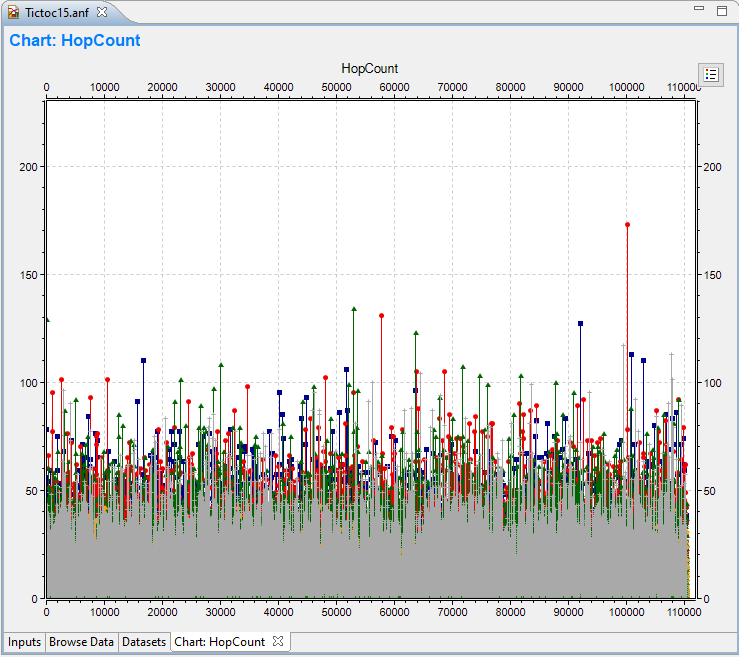
\includegraphics[scale=0.34]{images/plot-data.png}

	\item Pada \textit{background chart}, klik kanan \codeword{Properties}. Pada tab \codeword{Lines} kita dapat memilih \textit{Line type} dan \textit{Symbol type}. Pilih \codeword{Dots}
	\item Selanjutnya \textit{Display Legend} dengan cara, pilih menu \codeword{Legend} \textit{Display Legend}. \textit{Position above} dan \textit{Anchoring north}. Klik \textit{Ok}
\end{enumerate}

\subsection{Part 7: Parameter Studies}
Kita dapat menganalisis data yang sudah di \textit{record} dengan membuka \textit{file} yang berektensi \textit{.anf} , lalu pada tab \textit{Datasets} dapat dilihat dataset yang terdaftar.
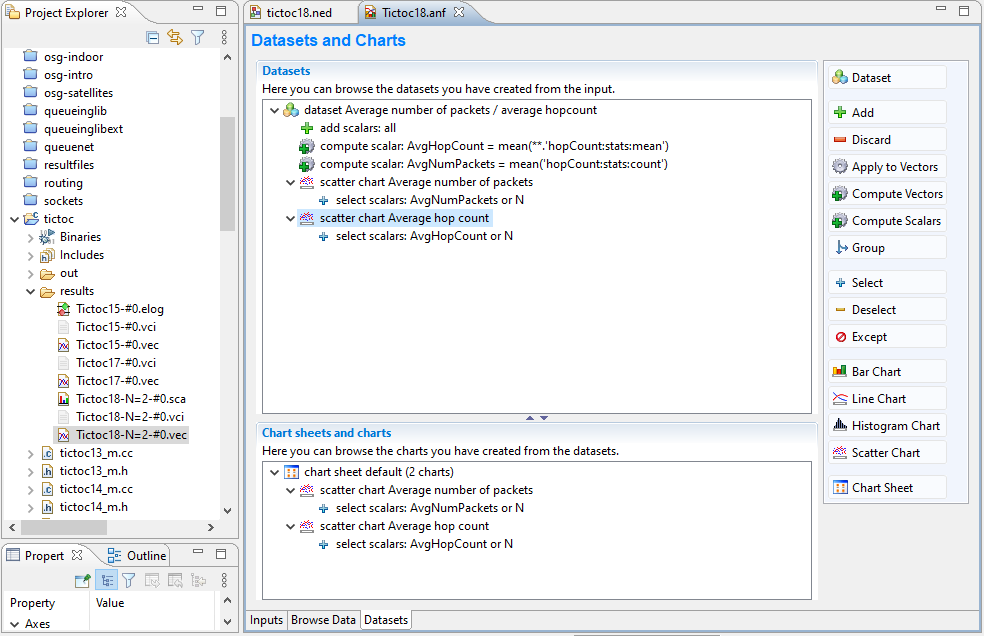
\includegraphics[scale=0.18]{images/tictoc18-analysis-file.png}

\section{Hasil dan Pembahasan}
Algoritma Dijkstra ini menentukan jalur tersingkat untuk sampai ke tujuan.Node menerima paket dari node sebelumnya dan menentukan akan kemana paket itu diteruskan

\section{Kesimpulan}
Algoritma Dijkstra ini menentukan jalur tersingkat untuk sampai ke tujuan

\bibliographystyle{./bibliography/IEEEtran}
\begin{thebibliography}{1}
	\bibitem{Installation Guide}\url{https://doc.omnetpp.org/omnetpp/InstallGuide.pdf}
	\bibitem{OMNet++ TicToc tutorial}\url{https://docs.omnetpp.org/tutorials/tictoc}
	\bibitem{User Guide}\url{https://doc.omnetpp.org/omnetpp/UserGuide.pdf}
\end{thebibliography}

\end{document}
